% Blueprint slides: organising the talk, not the final deck.
% Compile: pdflatex blueprint.tex
\documentclass[10pt,aspectratio=169]{beamer}

\usetheme{metropolis}
\usepackage{amsmath, amssymb}
\usepackage{bm}
\usepackage{booktabs}
\usepackage{multirow}
\usepackage[table]{xcolor}
\usepackage{tikz}
\usetikzlibrary{arrows.meta, positioning, fit, backgrounds}

\title{Differentiable Particle Filtering for Bayesian SSM Inference}
\subtitle{HMC + LEDH-invertible + OT resampling}
\author{Haowu Duan}
\date{\today}

\newcommand{\R}{\mathbb{R}}
\newcommand{\E}{\mathbb{E}}
\newcommand{\given}{\,|\,}
\newcommand{\Tmap}{\mathcal{T}}

\begin{document}

\maketitle

\begin{frame}{Roadmap}
  \tableofcontents
\end{frame}

% ============================================================
\section{Big picture: HMC + OT + LEDH-invertible}
% ============================================================

\begin{frame}{The problem we are solving}
  \textbf{Bayesian inference for state-space models.}
  \begin{align*}
    x_t &= f_\theta(x_{t-1},\, \eta_t) \\
    z_t &= h_\theta(x_t,\, \varepsilon_t)
  \end{align*}

  Given $z_{1:T}$, recover the posterior $p(\theta \given z_{1:T}) \propto p(z_{1:T}\given\theta)\,p(\theta)$.

  \medskip
  \textbf{The hard piece:} $p(z_{1:T}\given\theta)$ has no closed form for nonlinear / non-Gaussian models (stochastic volatility, range-bearing tracking).
\end{frame}

\begin{frame}{Our approach}
  \begin{itemize}\setlength{\itemsep}{1.2em}
    \item LEDH-invertible particle flow particle filter for the proposal.
    \item Optimal transport (Sinkhorn) resampling to make $p(z_{1:T}\given\theta)$ differentiable in $\theta$.
    \item Hamiltonian Monte Carlo to explore the posterior, validated on 1D linear Gaussian, 1D stochastic volatility, and range-bearing.
  \end{itemize}
\end{frame}

% ============================================================
\section{Sequential Monte Carlo and LEDH-invertible}
% ============================================================

\begin{frame}{Filtering as integration}
  Filtering does not need the whole posterior $p(x_t \given z_{1:t})$ --- it needs \textbf{moments}:
  \[
    \E[f(x_t) \given z_{1:t}] \;=\; \int f(x_t)\, p(x_t \given z_{1:t})\, dx_t,
  \]
  in particular the mean $m_t$ and covariance $P_t$.

  \medskip
  The recursion
  \[
    p(x_t \given z_{1:t}) \;\propto\; p(z_t \given x_t) \int p(x_t \given x_{t-1})\, p(x_{t-1} \given z_{1:t-1})\, dx_{t-1}
  \]
  is a \textbf{high-dimensional path integral}. Closed-form only in the linear-Gaussian case (Kalman). Otherwise intractable.

  \medskip
  \textbf{Particle methods are an integration scheme.} Represent the filtering distribution by weighted samples $\{(x_t^i, w_t^i)\}_{i=1}^N$, $\sum_i w_t^i = 1$. Any moment becomes a weighted sum:
  \[
    \E[f(x_t) \given z_{1:t}] \;\approx\; \sum_i w_t^i\, f(x_t^i).
  \]
\end{frame}

\begin{frame}{Sequential Monte Carlo --- the recipe}
  At step $t$, given $\{(x_{t-1}^i, w_{t-1}^i)\}$ approximating $p(x_{t-1} \given z_{1:t-1})$ with $\sum_i w_{t-1}^i = 1$:
  \begin{enumerate}\setlength{\itemsep}{0.3em}
    \item \textbf{Propagate} from any proposal: $x_t^i \sim q(\cdot \given x_{t-1}^i, z_t)$.
    \item \textbf{Reweight} (unnormalised):
    \[
      \tilde w_t^i \;=\; w_{t-1}^i \cdot \dfrac{p(z_t\given x_t^i)\, p(x_t^i\given x_{t-1}^i)}{q(x_t^i \given x_{t-1}^i, z_t)}.
    \]
    \item \textbf{Normalise:} $w_t^i \;=\; \tilde w_t^i \,/\, \sum_j \tilde w_t^j$.
    \item \textbf{Resample} when $\mathrm{ESS} < 0.5\, N$.
  \end{enumerate}

  \medskip
  Marginal likelihood --- the integral $\int p(z_{1:T}, x_{1:T}\given\theta)\, dx_{1:T}$ --- estimated by
  \[
    \log p(z_{1:T}\given\theta) \;=\; \sum_{t=1}^T \log\!\left(\sum_i \tilde w_t^i\right).
  \]
  Unbiased in $p$, but \textbf{noisy and non-smooth in $\theta$} when resampling is multinomial.
\end{frame}

\begin{frame}{Why the standard PF gradient hurts HMC}
  Two problems for $\nabla_\theta \log p$:
  \begin{itemize}
    \item \textbf{Resampling kills the gradient.} Multinomial / systematic resampling chooses indices --- discrete, non-differentiable. The score-function trick gives high-variance gradients.
    \item \textbf{Bootstrap proposal is wasteful.} $q = p(\cdot\given x_{t-1})$ ignores $z_t$; weights collapse, ESS crashes, variance of $\nabla_\theta$ explodes.
  \end{itemize}

  \medskip
  Two problems, two fixes:
  \begin{center}
  \begin{tabular}{ll}
    \toprule
    Better proposal $\rightarrow$ & LEDH flow (this section) \\
    Differentiable resample $\rightarrow$ & OT (next section) \\
    \bottomrule
  \end{tabular}
  \end{center}
\end{frame}

\begin{frame}{LEDH flow: the idea}
  Bayesian update at step $k$:
  \[
    p(x_k \given z_{1:k}) \;\propto\; \underbrace{p(x_k \given z_{1:k-1})}_{g(x)} \cdot \underbrace{p(z_k \given x_k)}_{h(x)}.
  \]
  BPF handles this by reweighting $g$ by $h$ --- the source of weight degeneracy. Daum--Huang takes the other route: \textbf{move the particles} via a deterministic flow that transports samples of $g$ into samples of $g h$.

  \medskip
  Pseudo-time $\lambda \in [0,1]$, \textbf{log-homotopy}:
  \[
    \log p(x, \lambda) = \log g(x) + \lambda \log h(x), \qquad p(\cdot, 0) = g, \;\; p(\cdot, 1) \propto g h.
  \]
  Particles obey $dx/d\lambda = f(x, \lambda)$. The induced density evolution is the \textbf{(zero-diffusion) Fokker--Planck / continuity equation}:
  \[
    \frac{\partial p}{\partial \lambda} = -\nabla \cdot (p f).
  \]
\end{frame}

\begin{frame}{LEDH flow: the implementation}
  Many flows $f$ satisfy the continuity equation. Pick a tractable one: \textbf{affine ansatz} with a Gaussian assumption for $p(x, \lambda)$.

  \medskip
  \textbf{Affine ansatz.} $f(x, \lambda) = A(\lambda)\, x + b(\lambda)$.

  \medskip
  Plugging into the Fokker--Planck constraint with the Gaussian assumption $p(x, \lambda) \sim \mathcal{N}(\bar\eta_\lambda, P_\lambda)$ and matching the precision evolution $P_\lambda^{-1} = P^{-1} + \lambda H^\top R^{-1} H$ gives a closed form:
  \[
    A(\lambda) = -\tfrac{1}{2} P\, H^\top (\lambda H P H^\top + R)^{-1} H,
    \quad
    b(\lambda) = (I + 2\lambda A)\big[(I + \lambda A) P H^\top R^{-1} z + A \bar\eta_0\big].
  \]
  $H = \partial h_\theta / \partial x$ is the observation-function Jacobian.

  \medskip
  \textbf{LEDH (vs.\ EDH).} Re-evaluate $H^{(i)} = \partial h_\theta / \partial x \big|_{x^{(i)}(\lambda)}$ at \emph{each particle's own current position} at every $\lambda$ step. Each particle gets its own $A^{(i)}(\lambda)$, $b^{(i)}(\lambda)$.

\end{frame}

\begin{frame}{Why invertibility matters here}
  \textbf{Invertible variant.} Track the Jacobian along the trajectory:
  \[
    J_t^i = \prod_{k} (I + \Delta\lambda\, A_{\lambda_k}^{(i)}).
  \]
  Weight update uses $\log|\det J_t^i|$ instead of a free proposal density.

  \medskip
  \begin{itemize}
    \item Free proposal $q$: weight ratio needs $q(x_t\given x_{t-1}, z_t)$, which we do not have for a flow.
    \item Invertible flow: $\log|\det J_t^i|$ enters the weight update via change-of-variables, accounting for the discretisation error the flow introduces in the measure.
    \item $J_t^i$ is differentiable in $\theta$. So the entire propagation step contributes a clean $\nabla_\theta$.
  \end{itemize}

  \medskip
  \textbf{Practical note.} TF's standard log-determinant routine swaps matrix rows around as it computes; JIT compilation on CPU does not know how to handle that pattern, so it errors. We compute $\log|\det J|$ from a QR factorisation instead --- no row-swapping, JIT-friendly on every backend.
\end{frame}

\begin{frame}{LEDH-PF in this codebase}
  \begin{itemize}
    \item Filter takes $\theta$ as an explicit tensor input, never as a captured constant. This avoids retracing on every HMC proposal.
    \item Inner loop over $T \times n_\lambda$ is a graph-mode while-loop, so $T$ becoming dynamic does not retrace.
    \item Diagnostics use graph-mode tensor arrays, not Python lists. Logging does not break the trace.
    \item Test coverage: dedicated JIT-compile and value-and-gradient suites.
  \end{itemize}

  \medskip
  \textbf{Status:} forward and gradient verified. JIT speedup $\sim 1.3\times$ forward at $T{=}20$. Throughput is dominated by $T \times n_\lambda \times N$, not framework overhead, except in 1D/2D models.
\end{frame}

% ============================================================
\section{OT resampling, Sinkhorn, and the neural operator}
% ============================================================

% ---------- Part 1: Why we need OT resampling ----------
\begin{frame}{Two problems with classical resampling}
  Resampling should change the particle representation \emph{without} changing the distribution it represents. Classical schemes have two failure modes.

  \medskip
  \textbf{Problem 1 --- sampling noise.}
  Multinomial / systematic resampling draws indices from $\mathbf{w}$. The selection itself injects extra Monte-Carlo noise on top of the filter's own variance. Sample impoverishment kills covariance estimates.

  \medskip
  \textbf{Problem 2 --- non-differentiability.}
  Picking discrete indices is not differentiable in any input. Standard linear-program OT solvers fix Problem 1 (deterministic) but not Problem 2 (LP plan has no derivatives w.r.t.\ inputs).

  \medskip
  Entropy-regularised OT (next slides) addresses both: deterministic transport map, differentiable in $(\mathbf{x}, \mathbf{w})$.
\end{frame}

% ---------- Part 2: Reich + what OT does ----------
\begin{frame}{Reich's framing of resampling}
  \textbf{Reich (2013), \emph{A nonparametric ensemble transform method for Bayesian inference} (SIAM J.\ Sci.\ Comput.\ 35(4)).} Treat resampling as a \emph{transport} problem. Pre-resample weighted cloud $\{(x_i, w_i)\}$, target equal-weight cloud $\{(\hat x_i, 1/N)\}$.

  \medskip
  Solve the discrete OT with marginals
  \[
    \mathbf{a} = \mathbf{w}, \qquad \mathbf{b} = \tfrac{1}{N}\mathbf{1}_N, \qquad C_{ij} = \tfrac{1}{2}\|x_i - x_j\|^2.
  \]
  Optimal coupling $\mathbf{P}^*$ has row sums $\mathbf{w}$ (source), column sums $\tfrac{1}{N}\mathbf{1}_N$ (target).

  \medskip
  \textbf{Resampled particle = column-weighted barycentre:}
  \[
    \hat x_i \;=\; N \sum_j P^*_{ji}\, x_j \;=\; \sum_j T_{ij}\, x_j,
    \qquad T_{ij} = N\, P^*_{ji}.
  \]
  Each new particle is a convex combination of the old ones. \textbf{No discrete selection} --- every input particle contributes to every output particle through $T_{ij}$.

  \medskip
  This is the gateway to differentiability: $T$ depends smoothly on $(\mathbf{x}, \mathbf{w})$ via the Sinkhorn solve.
\end{frame}

\begin{frame}{Reich's consistency theorem}
  \textbf{Why is the output a faithful sample of the underlying target $q$?}

  \medskip
  Sinkhorn itself is agnostic --- give it any $(\mathbf{a}, \mathbf{b}, \mathbf{C})$ and it returns the OT plan. The reason the resampled cloud is asymptotically a realisation of $q$ is a consistency result.

  \medskip
  \fbox{\parbox{0.95\textwidth}{
  \small
  \textbf{Theorem (Reich, \emph{A nonparametric ensemble transform method for Bayesian inference}, 2013).} Particles $x^{(1)}, \dots, x^{(N)}$ i.i.d.\ from proposal $q_{\text{prop}}$, importance weights $w_i \propto q(x^{(i)})/q_{\text{prop}}(x^{(i)})$. Let $\mathbf{P}^*$ be the unregularised OT plan with marginals $(\mathbf{w}, \tfrac{1}{N}\mathbf{1})$ and $L^2$ cost. Define $\hat x^{(i)} = N \sum_j P^*_{ji} x^{(j)}$. Then for every continuous bounded $f$,
  \[
    \tfrac{1}{N} \sum_i f(\hat x^{(i)}) \;\xrightarrow{N\to\infty}\; \int f\, dq \quad \text{a.s.}
  \]
  Equivalently, $\tfrac{1}{N}\sum_i \delta_{\hat x^{(i)}} \rightharpoonup q$ weakly.
  }}
\end{frame}

% ---------- Part 3: Sinkhorn + convergence ----------
\begin{frame}{Vanilla Sinkhorn --- where the iteration comes from}
  \textbf{Setup.} Two probability vectors $\mathbf{a} \in \Sigma_M$, $\mathbf{b} \in \Sigma_N$. Coupling matrices
  \[
    \mathcal{U}(\mathbf{a}, \mathbf{b}) = \{\,\mathbf{P} \in \R^{M\times N}_{+} \,:\, \mathbf{P}\mathbf{1}_N = \mathbf{a},\; \mathbf{P}^\top \mathbf{1}_M = \mathbf{b}\,\}.
  \]
  Entropic-regularised OT (Cuturi 2013):
  \[
    \min_{\mathbf{P} \in \mathcal{U}(\mathbf{a}, \mathbf{b})} \langle \mathbf{P}, \mathbf{C}\rangle - \varepsilon \mathbf{H}(\mathbf{P}),
    \qquad \mathbf{H}(\mathbf{P}) = -\!\sum_{ij} \mathbf{P}_{ij}(\log \mathbf{P}_{ij} - 1).
  \]
  \textbf{KKT.} Lagrangian $\mathcal{L} = \langle \mathbf{P}, \mathbf{C}\rangle - \varepsilon \mathbf{H} - \langle \mathbf{f}, \mathbf{P}\mathbf{1}_N - \mathbf{a}\rangle - \langle \mathbf{g}, \mathbf{P}^\top \mathbf{1}_M - \mathbf{b}\rangle$. Setting $\partial \mathcal{L}/\partial \mathbf{P}_{ij} = 0$:
  \[
    \mathbf{P}_{ij} = \exp\!\left(\tfrac{\mathbf{f}_i}{\varepsilon}\right)\,\exp\!\left(-\tfrac{\mathbf{C}_{ij}}{\varepsilon}\right)\,\exp\!\left(\tfrac{\mathbf{g}_j}{\varepsilon}\right)
    \;=\; \mathbf{u}_i\, \mathbf{K}_{ij}\, \mathbf{v}_j.
  \]
  \footnotesize Derivation: Xie (2025), \emph{Deriving the Gradients of Some Popular OT Algorithms} (arXiv:2504.08722), Prop.\ 3.
\end{frame}

\begin{frame}{Vanilla Sinkhorn --- the algorithm}
  In index notation, the marginal constraints
  $\sum_j P_{ij} = a_i$ and $\sum_i P_{ij} = b_j$ on $P_{ij} = u_i K_{ij} v_j$ give
  \[
    u_i\, K_{ij}\, v_j \;=\; a_i \quad (\text{sum on } j), \qquad
    v_j\, K_{ij}\, u_i \;=\; b_j \quad (\text{sum on } i),
  \]
  which solve to
  \[
    u_i \;=\; \frac{a_i}{K_{ij}\, v_j}, \qquad v_j \;=\; \frac{b_j}{K_{ij}\, u_i}.
  \]

  \medskip
  \begin{center}
  \fbox{\parbox{0.85\textwidth}{
  \footnotesize
  \textbf{Algorithm} (Vanilla Sinkhorn, Xie 2025, Alg.\ 3.1)\\[2pt]
  \textbf{Input:} $a_i, b_j, C_{ij}, \varepsilon > 0$. \quad \textbf{Init:} $u_i = 1$, $v_j = 1$. \quad $K_{ij} = \exp(-C_{ij}/\varepsilon)$.\\[2pt]
  \textbf{Repeat until convergence:} $\quad u_i \leftarrow a_i / (K_{ij}\, v_j)$; $\quad v_j \leftarrow b_j / (K_{ij}\, u_i)$.\\[2pt]
  \textbf{Output:} $P_{ij} = u_i\, K_{ij}\, v_j$.
  }}
  \end{center}

  \medskip
  Stopping criterion: $|u_i^{(L)} K_{ij} v_j^{(L)} - a_i| \le \rho$ and $|v_j^{(L)} K_{ij} u_i^{(L)} - b_j| \le \rho$ for every free index.
\end{frame}

\begin{frame}{Convergence of vanilla Sinkhorn}
  \textbf{Why it converges.}
  The entropic OT objective $\langle \mathbf{P}, \mathbf{C}\rangle - \varepsilon\, \mathbf{H}(\mathbf{P})$ is $\varepsilon$-strongly convex in $\mathbf{P}$ over the polytope $\mathcal{U}(\mathbf{a}, \mathbf{b})$. Strong convexity ensures a unique solution.

  \medskip
  Marginal violation $\max_i |u_i^{(\ell)} K_{ij} v_j^{(\ell)} - a_i|$ vs.\ iteration $\ell$, $N = 200$:

  \begin{center}
  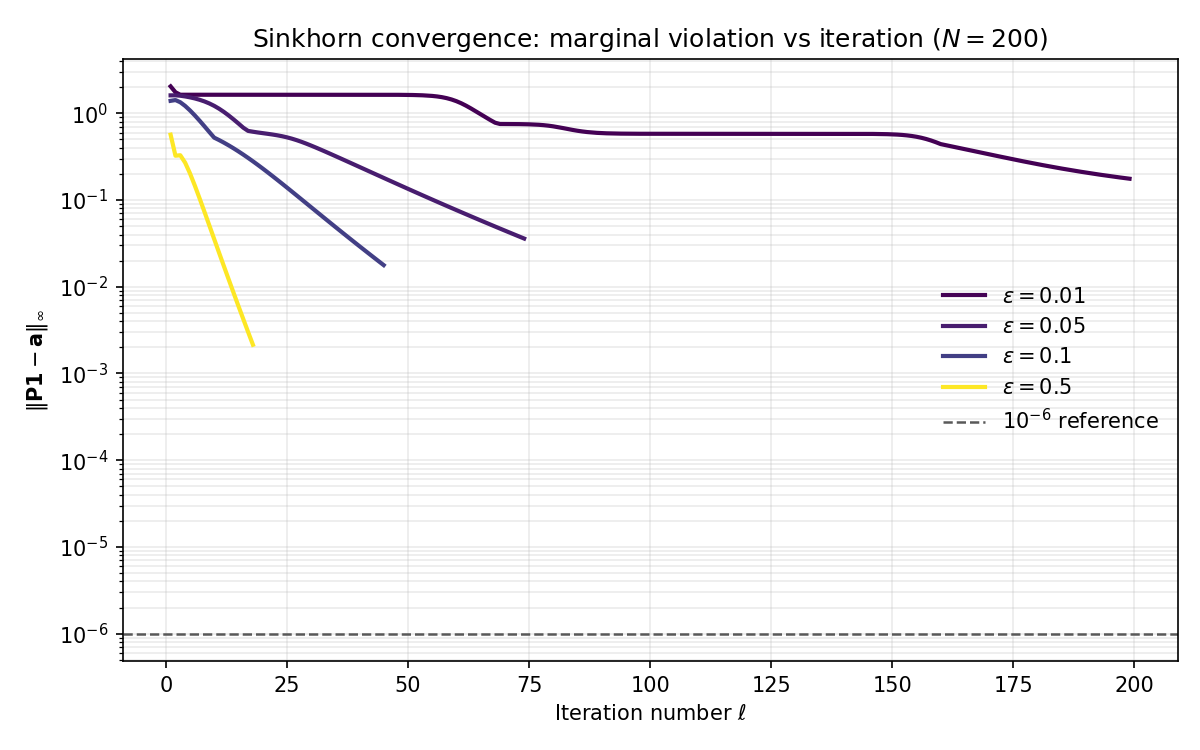
\includegraphics[height=0.55\textheight,keepaspectratio]{../report/sinkhorn_convergence.png}
  \end{center}
\end{frame}

\begin{frame}{Sharp vs blurry transport: $P_{ij}$ at small and large $\varepsilon$}
  Same $N = 50$ source/target on the line, particles sorted by position. Plot the converged $P_{ij}$:

  \begin{center}
  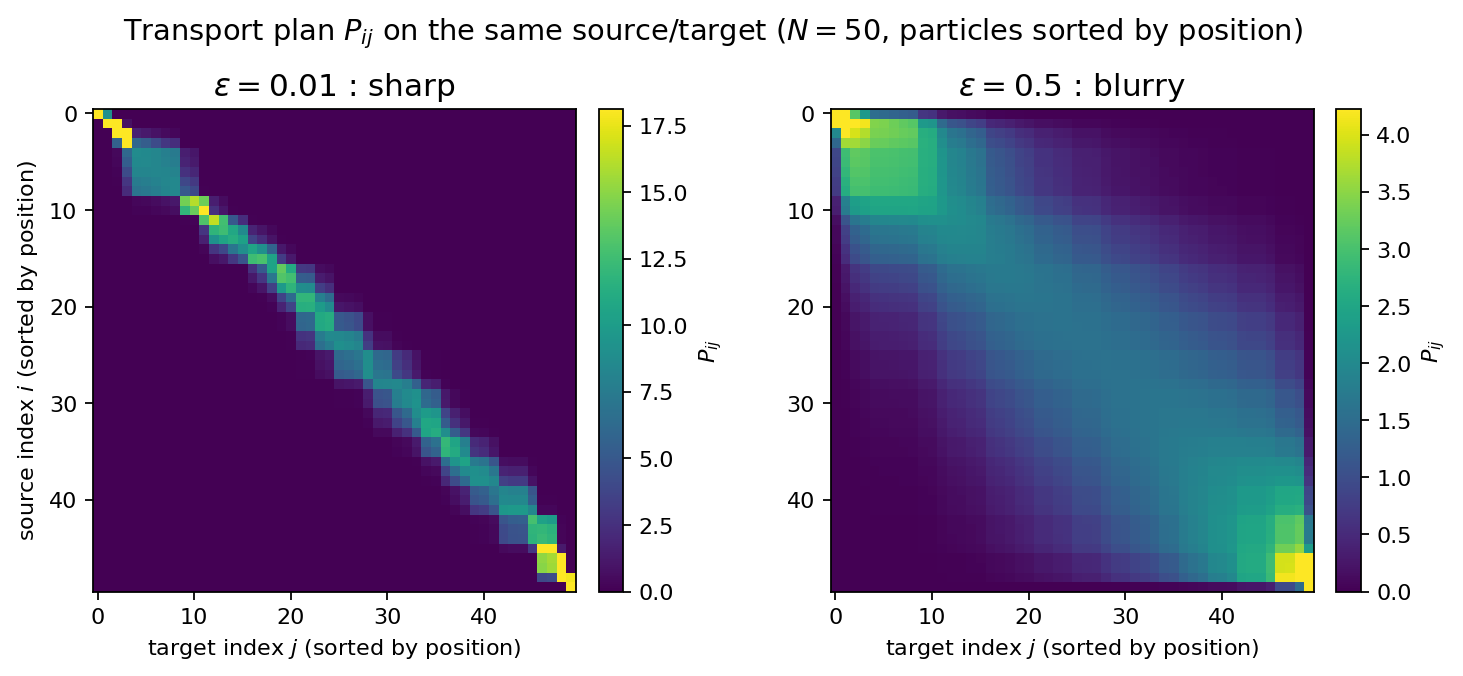
\includegraphics[width=0.95\linewidth]{figures/sinkhorn_heatmap.png}
  \end{center}
 \end{frame}

% ---------- Part 4: Implementation tricks ----------
\begin{frame}{Numerical instability: log-stabilised Sinkhorn}
  \textbf{The problem.} $K_{ij} = \exp(-C_{ij}/\varepsilon)$ underflows to $0$ when $C_{ij}/\varepsilon$ is large. Then $u_i, v_j$ explode in the divisions. Vanilla Sinkhorn breaks for spread-out clouds or small $\varepsilon$.

  \medskip
  \textbf{Fix.} Move to dual potentials $\alpha_i = \varepsilon \log u_i$, $\beta_j = \varepsilon \log v_j$. Then
  \[
    P_{ij} \;=\; \exp\!\left(\frac{\alpha_i + \beta_j - C_{ij}}{\varepsilon}\right),
  \]
  and the marginal-matching iteration becomes log-sum-exp (softmin):
  \[
    \alpha_i^\text{new} \;=\; -\varepsilon \log\!\sum_j \exp\!\left(\frac{\log b_j + \beta_j - C_{ij}}{\varepsilon}\right),
    \quad
    \beta_j^\text{new} \;=\; -\varepsilon \log\!\sum_i \exp\!\left(\frac{\log a_i + \alpha_i - C_{ij}}{\varepsilon}\right).
  \]
  Subtract row/column max before exponentiating $\Rightarrow$ numerically stable.

  \medskip
  \textbf{Damping for stability:} $\alpha_i \leftarrow \tfrac{1}{2}(\alpha_i + \alpha_i^\text{new})$, same for $\beta_j$. Trades one iteration's slowdown for monotone convergence on hard instances.
\end{frame}

% ---------- Part 5: Show the bias, fix it, show it's gone ----------

% --- Step 1: show the gradient bias ---

\begin{frame}{How we compute the reference gradient (FD)}
  \textbf{Central finite differences at multiple radii.} For parameter value $\theta_0$ and base step $h = 10^{-4}$:
  \[
    s_k \;=\; \frac{L(\theta_0 + k h) - L(\theta_0 - k h)}{2 k h}, \qquad k = 1, 2, 3, 4, 5
  \]
  \[
    \widehat{g}_\text{FD}(\theta_0) \;=\; \mathrm{median}\{s_1, \dots, s_5\}
  \]
  \textbf{Median, not mean} --- robust to one slope being polluted by a discontinuity / cliff. We also keep the five raw $s_k$: if they disagree, the function isn't smooth at $\theta_0$ and the FD gradient itself is suspect.

  \medskip
  \textbf{Autodiff side.} Reverse-mode autodiff of $L(\theta)$ at the same $\theta_0$.

  \medskip
  \textbf{Both sides use the same fixed PF seed} so randomness is deterministic. FD and autodiff measure the gradient of the \emph{same} numerical function, not two stochastic estimates.
\end{frame}

\begin{frame}{Filter-level bias compounds}
  \textbf{What is tested.} Linear-Gaussian SSM ($F{=}0.9$, $H{=}1$, true $\sigma_\text{obs}{=}1$). LEDH-PF with OT resampling ($\varepsilon{=}0.5$), $N{=}200$, $n_\lambda{=}15$, always-resample (no ESS gating), fixed PF seed.

  \medskip
  \textbf{Quantity:} $L(\theta) = \log p(z_{1:T}\given \sigma_\text{obs}{=}\theta)$, perturbed at $\theta_0 = 1.0$.

  \medskip
  Same code path, same forward, same FD. The only switch is which OT backward is plugged in.

  \medskip
  \begin{center}
  \footnotesize
  \begin{tabular}{r l r r l}
    \toprule
    $T$ & Backward & FD median $\widehat{g}_\text{FD}$ & Autodiff $\widehat{g}_\text{AD}$ & Verdict \\
    \midrule
    1  & approx   & $\phantom{-}0.008925$ & $\phantom{-}0.008924$ & rel.err.\ $9.3{\times}10^{-5}$ \\
    1  & implicit & $\phantom{-}0.008925$ & $\phantom{-}0.008924$ & rel.err.\ $9.3{\times}10^{-5}$ \\
    \midrule
    \rowcolor{red!15}
    5  & approx   & $-1.2902$              & $\phantom{-}\mathbf{+0.3690}$ & \textbf{wrong sign}, rel.err.\ $1.286$ \\
    5  & implicit & $-1.2902$              & $-1.2890$             & rel.err.\ $9.4{\times}10^{-4}$ \\
    \midrule
    20 & implicit & $\phantom{-}7.9400$    & $\phantom{-}7.9440$   & rel.err.\ $5.1{\times}10^{-4}$ \\
    \bottomrule
  \end{tabular}
  \end{center}

  \medskip
  \footnotesize Sources: \texttt{test\_gradient\_vs\_numerical\_lg\_ot\_approx.json}, \texttt{test\_gradient\_vs\_numerical\_lg.json}.
\end{frame}

\begin{frame}{The five FD slopes at $T{=}5$ --- why this is damning}
  Same case, $T{=}5$, $\theta_0 = 1.0$. The five central-difference slopes at radii $h, 2h, 3h, 4h, 5h$:

  \medskip
  \begin{center}
  \footnotesize
  \begin{tabular}{r l}
    \toprule
    $k$ & $s_k = \big(L(\theta_0 + kh) - L(\theta_0 - kh)\big)/(2kh)$ \\
    \midrule
    1 & $-1.290228679264871$ \\
    2 & $-1.290228676813498$ \\
    3 & $-1.290228672763405$ \\
    4 & $-1.290228667085724$ \\
    5 & $-1.290228659785342$ \\
    \midrule
    median & $\widehat{g}_\text{FD} = -1.2902286727634047$ \\
    \bottomrule
  \end{tabular}
  \end{center}

  \medskip
  Five slopes agreeing to seven decimal places $\Rightarrow$ $L(\theta)$ is smooth at $\theta_0$, the true gradient is unambiguously $\approx -1.2902$.

  \medskip
  Autodiff returns:
  \begin{itemize}
    \item Approximate backward: $\widehat{g}_\text{AD} = +0.3690$ \quad ($\Rightarrow$ \textbf{sign and magnitude both wrong})
    \item Implicit backward: $\widehat{g}_\text{AD} = -1.2890$ \quad ($\Rightarrow$ matches FD to $9.4 \times 10^{-4}$)
  \end{itemize}

  \medskip
  No way to blame stochasticity, no way to blame discontinuity. The bias is in the backward formula.
\end{frame}

% --- Step 2: introduce implicit gradient ---

\begin{frame}{Implicit backward: don't assume exact convergence}
  At convergence the Sinkhorn iterates $(u_i, v_j)$ satisfy the marginal-matching system
  \[
    F(u, v;\, a, C) \;=\; \begin{pmatrix} u_i K_{ij} v_j - a_i \\ v_j K_{ij} u_i - b_j \end{pmatrix} \;=\; 0.
  \]
  In practice we early-stop, so $F = r \neq 0$.

  \medskip
  \textbf{Approximate (extrapolation) backward.} Pretends $r = 0$. Treats $(u^*, v^*)$ as an exact fixed point and reads gradients off one extra Sinkhorn step. Drops the residual.

  \medskip
  \textbf{Implicit backward.} Linearises $F$ at the actual returned $(u^*, v^*)$, residual and all. Implicit function theorem gives
  \[
    \frac{\partial(u^*, v^*)}{\partial(a, C)} \;=\; -\!\left(\frac{\partial F}{\partial(u, v)}\right)^{\!-1}\!\frac{\partial F}{\partial(a, C)},
  \]
  evaluated at the returned point. One $(2N{-}1)$ Cholesky-grade solve.
\end{frame}

% --- Step 3: show the bias has been removed ---

\begin{frame}{Validation: implicit backward across models}
  All rows: AD vs FD ratio of $d \log p(z_{1:T}\given\theta)/d\theta$ with the implicit Sinkhorn backward, $7$ cases per row ($T \in \{1, 5, 20\}$ at the nominal parameter, plus $4$ parameter values at $T = 20$).

  \medskip
  \begin{center}
  \footnotesize
  \begin{tabular}{l c c c c c}
    \toprule
    Filter--model & Cases & Parameter sweep & Median rel.\ err. & Max rel.\ err. & Pass \\
    \midrule
    LG, BPF$+$OT             & $7$ & $\sigma_\text{obs} \in \{0.5, 1.0, 1.5, 2.0\}$ & $1.2{\times}10^{-4}$ & $4.1{\times}10^{-4}$ & yes \\
    LG, LEDH$+$OT            & $7$ & $\sigma_\text{obs} \in \{0.5, 1.0, 1.5, 2.0\}$ & $5.1{\times}10^{-4}$ & $3.2{\times}10^{-3}$ & yes \\
    RB, LEDH$+$OT            & $7$ & $\sigma_\text{range} \in \{0.05, 0.1, 0.2, 0.5\}$ & $2.0{\times}10^{-4}$ & $1.4{\times}10^{-3}$ & yes \\
    SV1D, LEDH$+$OT          & $7$ & $\alpha \in \{0.5, 0.7, 0.91, 0.95\}$ & $6.5{\times}10^{-4}$ & $2.0{\times}10^{-3}$ & yes \\
    \bottomrule
  \end{tabular}
  \end{center}

  \medskip
  All rows pass with median rel.\ err.\ $< 10^{-3}$ and max $< 5\times 10^{-3}$. The implicit backward delivers FD-accurate gradients across BPF and LEDH on linear Gaussian, range-bearing, and SV1D.
\end{frame}

\begin{frame}{The cost wall}
  \begin{center}
  \begin{tabular}{lr}
    \toprule
    Component & Cost vs.\ multinomial \\
    \midrule
    OT forward (Sinkhorn) & 60--100$\times$ \\
    Implicit backward (per resample) & one $2N{-}1$ Cholesky solve \\
    Per HMC proposal & $L \cdot T \cdot$ (above) \\
    Per chain & $n_\text{samples} \cdot$ (above) \\
    \bottomrule
  \end{tabular}
  \end{center}

  \medskip
  Concretely: $L{=}10$, $n{=}500$, $T{=}50$ $\Rightarrow$ 250{,}000 resamples \emph{per chain}.

  \medskip
  Practical now for $T \le 100$, $d \le 2$. Impractical as $T, N, d$ grow.
\end{frame}

\begin{frame}{Why a neural operator?}
  \textbf{Amortisation.} A single HMC chain solves hundreds of thousands of \emph{nearby} OT problems. Sinkhorn restarts each from scratch.

  \medskip
  Train a map $\Tmap_W(x;\, c)$ once, where $c$ summarises the cloud. At inference:
  \begin{itemize}
    \item One forward pass per resample, no inner iteration.
    \item No $(2N{-}1) \times (2N{-}1)$ solve in the backward.
    \item $O(L \cdot N^2) \rightarrow O(N \cdot \text{forward\_cost})$.
  \end{itemize}

  \medskip
  \textbf{The case is purely about repeated cost.} Sinkhorn correctness is not at issue.
\end{frame}

\begin{frame}{Monge--Amp\`ere equation, intuitively}
  \textbf{Mass conservation under change of variables.} If a map $T : \R^d \to \R^d$ pushes density $p$ onto density $q$, then
  \[
    \boxed{\;p(x) \;=\; q(T(x)) \,\big|\det J_T(x)\big|\;}
  \]
  Reading: at every $x$, the source mass $p(x)\,dx$ must equal the target mass $q(T(x))\,dy$ in the image; the Jacobian determinant is the local volume-change factor.

  \medskip
  \textbf{Brenier's theorem.} For squared-Euclidean cost, the OT map has the form $T = \nabla\varphi$ with $\varphi$ convex. Substituting:
  \[
    p(x) \;=\; q\big(\nabla\varphi(x)\big)\, \det \nabla^2\varphi(x).
  \]
  This is the \emph{Monge--Amp\`ere equation} --- a fully nonlinear PDE for the potential $\varphi$.

  \medskip
  \textbf{Our route.} We do not solve the PDE for $\varphi$. We parameterise the \emph{map} $T(x; c)$ directly with a neural network and enforce the boxed identity above as a training residual. This skips the second-order Hessian of $\varphi$ and gives both $T$ and $J_T$ from one forward pass.
\end{frame}

\begin{frame}{Using Monge--Amp\`ere for resampling: build source and target}
  Resampling input: a weighted particle cloud $\{(x_i, w_i)\}_{i=1}^N$ approximating some distribution. We want to redistribute mass so the cloud becomes equally weighted.

  \medskip
  \textbf{Why we need smooth densities.} The change-of-variables identity $p(x) = q(T(x))\,|\det J_T|$ requires absolutely continuous $p, q$. Empirical clouds are atomic --- they don't fit. \textbf{Smooth them with a Gaussian KDE} (bandwidth $h$, $K_h(u) = (2\pi h^2)^{-d/2}\exp(-\|u\|^2/(2h^2))$).

  \medskip
  \textbf{Source $p_h$ --- the cloud as if uniformly weighted.}
  \[
    p_h(x) \;=\; \frac{1}{N} \sum_{i=1}^N K_h(x - x_i)
  \]

  \medskip
  \textbf{Target $q_h$ --- the cloud with the importance weights.}
  \[
    q_h(x) \;=\; \sum_{i=1}^N w_i\, K_h(x - x_i)
  \]
  Same particle locations, but mass concentrated where $w_i$ is large.

  \medskip
  Both live on the same support, differ only in mass distribution. The map $T(x;c)$ must satisfy $p_h(x) = q_h(T(x;c))\,|\det J_T(x;c)|$ --- pulling mass from the uniformly-weighted picture to the weighted one.
\end{frame}

\begin{frame}{Inputs and outputs of the operator}
  \textbf{Inputs.}
  \begin{itemize}\setlength{\itemsep}{0.2em}
    \item \textbf{Query point} $x \in \R^d$ (or a batch $(B, d)$ at training). The point at which we evaluate the map.
    \item \textbf{Context} $c \in \R^C$ summarising the weighted cloud $\{(x_i, w_i)\}_{i=1}^N$. Built by a permutation-invariant set encoder: per-particle tokens $t_i = [x_i, \log w_i, w_i]$, learned map, weighted pool $\sum_i w_i h_i$; joined with weighted mean, covariance, $\log N$, $\log \mathrm{ESS}$, $\log h$, then projected to $c$.
  \end{itemize}

  \medskip
  \textbf{Outputs.}
  \begin{itemize}\setlength{\itemsep}{0.2em}
    \item \textbf{Transported point} $T(x; c) \in \R^d$.
    \item \textbf{Local Jacobian} $J_T(x; c) \in \R^{d \times d}$ --- analytic, from the same forward pass (not autodiffed).
  \end{itemize}

  \medskip
  Both are produced together; the loss needs $|\det J_T|$ at every collocation point, so getting it from the same forward pass (instead of nesting an autodiff call) is the architectural priority.
\end{frame}

\begin{frame}{Combining with resampling: the inference path}
  At every resample step in the filter:
  \begin{enumerate}\setlength{\itemsep}{0.3em}
    \item Take the weighted cloud $\{(x_i, w_i)\}_{i=1}^N$.
    \item Encode it once: $c \;\leftarrow\; \mathrm{SetEncoder}(\{(x_i, w_i)\})$.
    \item Apply the trained map to every particle in parallel:
    \[
      \tilde x_i \;=\; T(x_i;\, c), \qquad \tilde w_i \;=\; 1/N.
    \]
    Return $J_T(x_i; c)$ as well, for covariance transport in the LEDH flow.
  \end{enumerate}

  \medskip
  Differentiability: $T(x; c)$ and $J_T(x; c)$ are smooth functions of their inputs; gradients flow through the cloud $\{(x_i, w_i)\}$ to $\theta$ exactly as before.
\end{frame}

\begin{frame}{Training loss --- self-supervised Monge--Amp\`ere residual}
  No Sinkhorn teacher: the loss is the residual of the Monge--Amp\`ere equation itself, evaluated at collocation points.

  \medskip
  \[
    r(x;c) \;=\; \log p_h(x) \;-\; \log q_h\!\big(T(x;c)\big) \;-\; \log\big|\det J_T(x;c)\big|
  \]
  \[
    \mathcal{L}_\text{MA}(c) \;=\; \E_{x \sim p_h}\!\left[r(x;c)^2\right]
  \]

  \medskip
  Plus two regularisers:
  \begin{itemize}\setlength{\itemsep}{0.2em}
    \item \textbf{Local linearity:} $\|T(x{+}\delta;c) - T(x;c) - J_T(x;c)\,\delta\|^2$ on the KDE scale. Low-pass with cutoff $1/h$.
    \item \textbf{Eigenvalue barrier:} penalises $\lambda_\text{min}(J_T)$ below threshold (keeps $J_T$ well-conditioned, $\det > 0$).
  \end{itemize}

  \medskip
  \textbf{Sinkhorn role.} No Sinkhorn at training; Sinkhorn results will be used for validation.
\end{frame}

\begin{frame}{How do we know training has converged?}
  \textbf{Status today.} Single-cloud overfit reaches $\mathcal{L}_\text{MA} \approx 9\times 10^{-4}$, mean transport error $0.035$. \emph{The operator can fit one cloud.} Generalisation is not yet validated end-to-end.

  \medskip
  \textbf{Three gating tests --- designed, not yet run.}
  \begin{enumerate}\setlength{\itemsep}{0.2em}
    \item \textbf{Held-out MA residual.} Train on a Gaussian-cloud family; evaluate $\mathcal{L}_\text{MA}$ on cloud configurations the operator never saw.
    \item \textbf{Resample quality vs.\ Sinkhorn.} On held-out clouds, compare the operator's resampled cloud to the Sinkhorn cloud: $\mathrm{KL}(T_\# p_h \,\|\, q_h)$ or Sinkhorn divergence.
    \item \textbf{Filter-level recovery.} Drop the operator into LEDH$+$OT on linear Gaussian; check posterior recovery against the Sinkhorn-baseline HMC. The end-to-end test.
  \end{enumerate}

  \medskip
  Until tests 1--3 pass, ``low training loss'' is not ``trained operator''. The dataset pipeline (100 Gaussian-grid clouds, 70/15/15 split) is the gating work.
\end{frame}

\begin{frame}{Determinant in higher dimension --- forward and backward}
  The concern: $\det J_T$ is $O(d^3)$ for a generic $d \times d$ matrix, and the derivative makes it worse. How do we keep this from blowing up?

  \medskip
  \textbf{Architectural fix --- structured Jacobian.} We never let $J_T$ be a generic dense matrix. We force the structure
  \[
    J_T(x; c) \;=\; \lambda(c)\, I \;+\; \sum_{m} W_m^\top D_m(x;c)\, W_m,
  \]
  with $D_m \succeq 0$ diagonal. By construction $J_T$ is symmetric PSD, so $\det J_T > 0$ and $\log|\det J_T| = \log\det J_T$ (no sign tracking).

  \medskip
  \textbf{Forward $\det$ via Cholesky.} $O(d^3)$ per query point in the worst case --- but trivial at $d \le 2$ (every model in this report).

  \medskip
  \textbf{Backward through $\log\det$.} The identity $\partial \log\det A / \partial A = A^{-\top}$. \emph{One linear solve, not a Hessian.} Cholesky factor from the forward is reused $\Rightarrow$ one triangular solve, same $O(d^3)$. The derivative is no harder than the forward.

  \medskip
  \textbf{Escape hatch for high $d$.} Take each $W_m$ to be rectangular $r \times d$ with $r \ll d$. Then $W_m^\top D_m W_m$ is a rank-$r$ update of $\lambda I$. Matrix-determinant lemma:
  \[
    \det(\lambda I + W^\top D W) \;=\; \lambda^d \cdot \det\!\big(I_r + W D W^\top / \lambda\big),
  \]
  collapsing the $d \times d$ determinant to an $r \times r$ one: $O(r^3 + rd)$ instead of $O(d^3)$. The same $A^{-\top}$ identity works in the backward.

  \medskip
  Bottom line: with structured $J_T$, the determinant scales linearly in $d$ for the high-dim case, not cubically. It is no longer the bottleneck.
\end{frame}

\begin{frame}{Should $\theta$ be an input?}
  \textbf{The case for adding $\theta$.} HMC moves $\theta$ every proposal; the cloud the filter produces depends on $\theta$. So in principle conditioning the operator on $\theta$ gives it more information.

  \medskip
  \textbf{Why we don't, by default.}
  \begin{itemize}\setlength{\itemsep}{0.2em}
    \item Different parametric families have different $\theta$. Conditioning ties the operator to one family --- breaks the goal of a model-agnostic operator.
    \item Even within one family, $\theta$ alone does \emph{not} pin down the cloud: at fixed $\theta$ the filter produces a \emph{different} cloud at every $t = 1, \dots, T$. Conditioning on $\theta$ is not sufficient information.
    \item The cloud $\{(x_i, w_i)\}$ already carries the effect of $\theta$. As long as the cloud is a sufficient summary, the operator does not need $\theta$.
  \end{itemize}

  \medskip
  \textbf{Precondition for adding $\theta$.} It would help only if two trajectories $\gamma_{\theta_1}, \gamma_{\theta_2}$ pass through clouds that look the same in $(x, w)$-space but require \emph{different} transport maps. Empirical check: scan held-out (cloud, target) pairs; if cloud-only residual correlates with $\theta$ at fixed $c$, the cloud is not sufficient and $\theta$ should be added. Until that check fails, cloud-only is the parsimonious default.
\end{frame}

\begin{frame}{JIT-compiling the operator inside HMC}
  \textbf{Why it's hard.}
  \begin{itemize}\setlength{\itemsep}{0.2em}
    \item The operator is a learned module with weights and (likely) Keras layers. Any single non-XLA kernel inside breaks the trace.
    \item Operator weights are \emph{frozen} at HMC time. If the trace records weight reads as gradient sources, autodiff traces through them needlessly.
    \item The full HMC graph stacks: filter forward $\to$ operator at every resample $\to$ analytic Jacobian $\to$ autodiff back to $\theta$. One non-XLA op anywhere kills the whole compilation.
    \item The training loss uses operations like \texttt{slogdet} and \texttt{eigvalsh}; the first has no XLA-CPU kernel, the second is brittle inside JIT.
  \end{itemize}

  \medskip
  \textbf{What we do.}
  \begin{itemize}\setlength{\itemsep}{0.2em}
    \item Single inner JIT-compiled function: filter forward $+$ operator calls $+$ analytic Jacobian $+$ autodiff back to $\theta$. Operator weights stop-gradient'd on weight reads (not outputs).
    \item Replace \texttt{slogdet} with the same QR-based log-abs-det used for LEDH.
    \item Drop training-only regularisers (eigenvalue barrier, local linearity) from the inference graph --- they are training-time only.
    \item Validate the same way as Sinkhorn: FD vs.\ autodiff of $\log p(z_{1:T} | \theta)$ with the operator in the loop. If FD ratio $\approx 1$, the path is JIT-clean.
  \end{itemize}
\end{frame}

% ============================================================
\section{HMC + LEDH + OT pipeline}
% ============================================================

\begin{frame}{The full pipeline}
  \begin{center}
  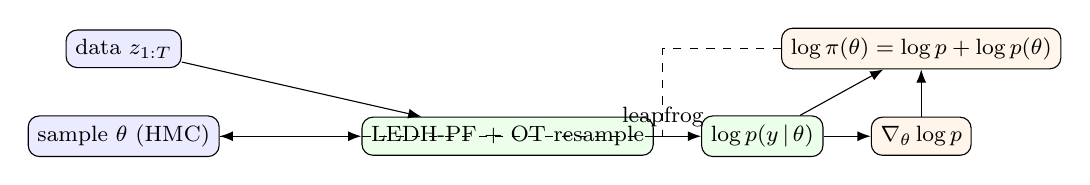
\begin{tikzpicture}[every node/.style={font=\footnotesize}, node distance=6mm]
    \node[draw, rounded corners, fill=blue!8] (data) {data $z_{1:T}$};
    \node[draw, rounded corners, below=of data, fill=blue!8] (theta) {sample $\theta$ (HMC)};
    \node[draw, rounded corners, right=18mm of theta, fill=green!8] (filter) {LEDH-PF $+$ OT resample};
    \node[draw, rounded corners, right=of filter, fill=green!8] (lik) {$\log p(y\given\theta)$};
    \node[draw, rounded corners, right=of lik, fill=orange!8] (grad) {$\nabla_\theta \log p$};
    \node[draw, rounded corners, above=of grad, fill=orange!8] (lp) {$\log\pi(\theta) = \log p + \log p(\theta)$};

    \draw[-Latex] (data) -- (filter);
    \draw[-Latex] (theta) -- (filter);
    \draw[-Latex] (filter) -- (lik);
    \draw[-Latex] (lik) -- (grad);
    \draw[-Latex] (lik) -- (lp);
    \draw[-Latex] (grad.north) -- (lp.south);
    \draw[-Latex, dashed] (lp.west) -- ++(-1.5,0) |- (theta.east) node[midway, above]{leapfrog};
  \end{tikzpicture}
  \end{center}

  \medskip
  All boxes inside one JIT-compiled graph; gradient computed by reverse-mode autodiff on the same trace.
\end{frame}

\begin{frame}{HMC setup --- the choices that matter}
  \begin{itemize}
    \item \textbf{Sampler:} Hamiltonian Monte Carlo with dual averaging on the step size; target acceptance 0.75--0.80.
    \item \textbf{Leapfrog:} $L = 10$ for SV1D / RB; per-axis step in RB.
    \item \textbf{Chains:} 4 independent, separate DA inits. (Single-chain ESS $= 4.0$ on SV1D was a DA-init artefact, not a real failure --- 4 chains converge.)
    \item \textbf{Bijectors} for the SVSSM:
    \begin{itemize}
      \item $\mu$: identity
      \item $\phi$: $\tanh$ ($\R \to (-1,1)$)
      \item $\sigma_\eta$: softplus
    \end{itemize}
    \item \textbf{Diagnostics:} split-$\hat R \le 1.01$ (Vehtari et al.\ 2021), bulk + tail ESS $\ge 100$ per parameter per chain, energy diagnostics.
  \end{itemize}
\end{frame}

\begin{frame}{Priors for the SVSSM}
  \begin{itemize}
    \item $\mu \sim \mathcal{N}(0, 5^2)$ --- weakly informative; log-volatility mean is negative for typical assets but should not be hard-bounded.
    \item $\phi \sim \mathrm{Beta}(20, 1.5)$ mapped to $(-1, 1)$ --- support concentrated near $0.95$--$0.99$, matches financial empirics.
    \item $\sigma_\eta \sim \mathrm{LogNormal}(\log\sigma_\eta^* + 0.25,\, 0.5)$ --- mode at the true value (LogNormal mode quirk: $\exp(\mu - s^2)$).
  \end{itemize}

  \medskip
  Why this matters for HMC: the prior's tail behaviour interacts with the bijector --- weakly identified directions can stretch the leapfrog trajectory past the typical set.
\end{frame}

\begin{frame}{Initial condition $h_0$}
  \textbf{Stationary} ($|\phi| < 1$):
  \[
    h_0 \sim \mathcal{N}\!\left(\mu,\, \frac{\sigma_\eta^2}{1 - \phi^2}\right)
  \]
  \textbf{Non-stationary} ($|\phi| \ge 1$): diffuse $h_0 \sim \mathcal{N}(0, \kappa)$ with large $\kappa$.

  \medskip
  \textbf{The trap.} The stationary form makes $\Sigma_0 = \sigma_\eta^2 / (1{-}\phi^2)$ a function of $(\phi, \sigma_\eta)$. Differentiating through the Cholesky $\to \exp$ chain explodes near $\phi \to 1$.

  \medskip
  \textbf{This codebase:} detach $h_0$ from transition parameters via numpy init. Slight prior bias, removes the gradient pathology that froze HMC at high persistence.
\end{frame}

% ---------- Benchmark pipeline: KF baseline → MAP sanity → HMC ----------

\begin{frame}{Benchmark step 1: linear-Gaussian HMC, Kalman / EKF / UKF}
  Same linear-Gaussian observation sequence ($\sigma_\text{obs}^* = 1.0$). Four chains each, dual averaging, target acceptance $0.65$.

  \medskip
  \begin{center}
  \footnotesize
  \begin{tabular}{l c c c c c c}
    \toprule
    Filter & Posterior mean & Sd & 90\% CI & Max $\hat R$ & Bulk ESS & Tail ESS \\
    \midrule
    Kalman & $1.127$ & $0.177$ & $[0.85,\, 1.44]$ & $1.008$ & $278$ & $325$ \\
    EKF    & $1.142$ & $0.176$ & $[0.87,\, 1.46]$ & $1.003$ & $419$ & $518$ \\
    UKF    & $1.138$ & $0.173$ & $[0.87,\, 1.45]$ & $1.002$ & $464$ & $494$ \\
    \bottomrule
  \end{tabular}
  \end{center}

  \medskip
  All three converge: $\max\hat R \le 1.008$ on rank-normalised samples, bulk + tail ESS in the hundreds. Posterior means agree to within $0.015$ on the same data; the $\sim 0.13$ offset above the truth is dataset-specific. This is the convergence target for the differentiable-filter HMC runs that follow.
\end{frame}

\begin{frame}{Diagnostics: ESS and rank-normalised $\hat R$}
  \textbf{Effective sample size (ESS).} For a chain of $N$ samples of a parameter $\theta$ with lag-$k$ autocorrelation $\hat\rho_k$,
  \[
    \mathrm{ESS} \;=\; \frac{N}{1 + 2 \sum_{k \ge 1} \hat\rho_k}.
  \]
  Counts effectively-independent samples. \textbf{Bulk ESS} is computed on the rank-normalised pooled samples; \textbf{tail ESS} on the indicators $\mathbb{1}\{\theta < q_{0.05}\}$ and $\mathbb{1}\{\theta > q_{0.95}\}$ (catches tail-mixing failures bulk ESS misses). Threshold: bulk + tail ESS $\ge 100$ per parameter per chain.

  \medskip
  \textbf{Rank-normalised $\hat R$ (Vehtari et al.\ 2021).} Pool all $MN$ samples, replace each by its rank, transform to standard normal: $z_t^{(m)} = \Phi^{-1}\!\big(\mathrm{rank}(\theta_t^{(m)})/(MN+1)\big)$. Run the standard between-/within-chain variance ratio on $z$:
  \[
    \hat R \;=\; \sqrt{\frac{\widehat{\mathrm{Var}}(z)}{W(z)}}, \qquad
    \widehat{\mathrm{Var}}(z) = \frac{N-1}{N} W(z) + \frac{1}{N} B(z).
  \]
  Rank normalisation makes the test sensitive to \emph{any} cross-chain distributional difference, not just mean/variance.

  \medskip
  \textbf{Bulk-$\hat R$ vs.\ tail-$\hat R$.} Bulk uses $z$ above; tail folds $\tilde\theta_t^{(m)} = |\theta_t^{(m)} - \mathrm{median}(\theta)|$ first, then rank-normalises and recomputes. We report $\max(\text{bulk-}\hat R, \text{tail-}\hat R)$ (Stan default). Convergence threshold: $\le 1.01$.
\end{frame}

\begin{frame}{Benchmark step 2: MAP sanity --- BPF$+$OT and LEDH$+$OT on LG}
  \begin{center}
  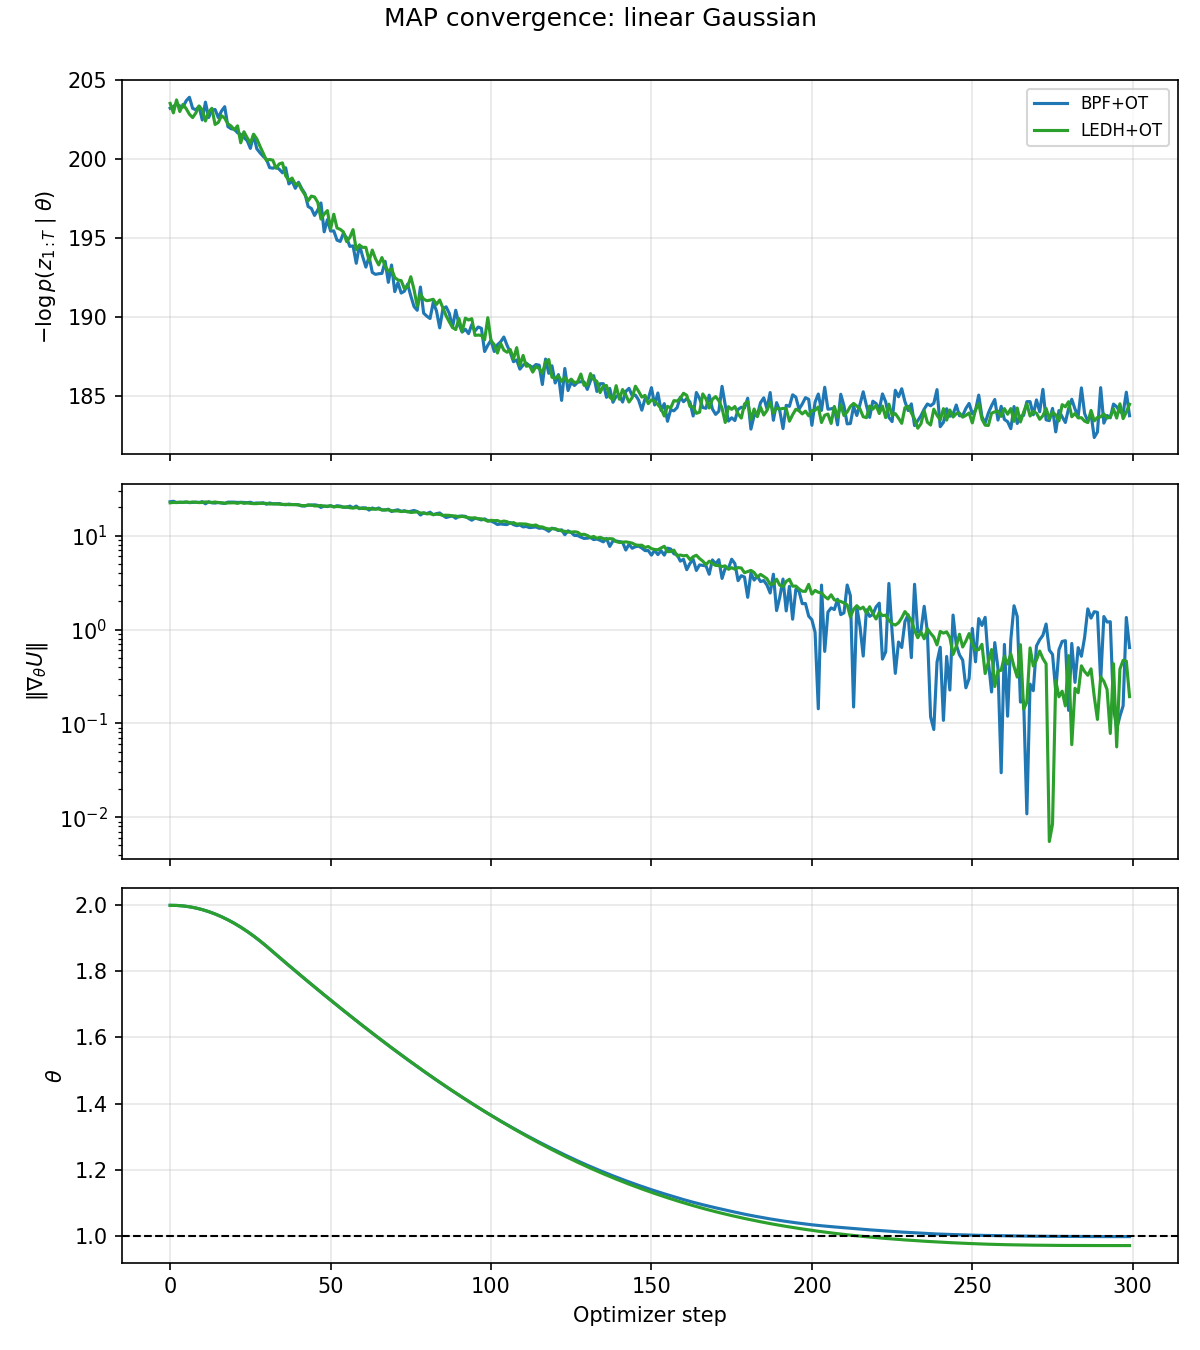
\includegraphics[height=0.78\textheight,keepaspectratio]{../report/map_lg.png}
  \end{center}
\end{frame}

\begin{frame}{Benchmark step 3: HMC on linear Gaussian}
  Same LG setup. Run HMC on $\sigma_\text{obs}$ with both BPF$+$OT and LEDH$+$OT, four chains each, separate dual-averaging inits. Compare to the Kalman family baseline.

  \begin{center}
  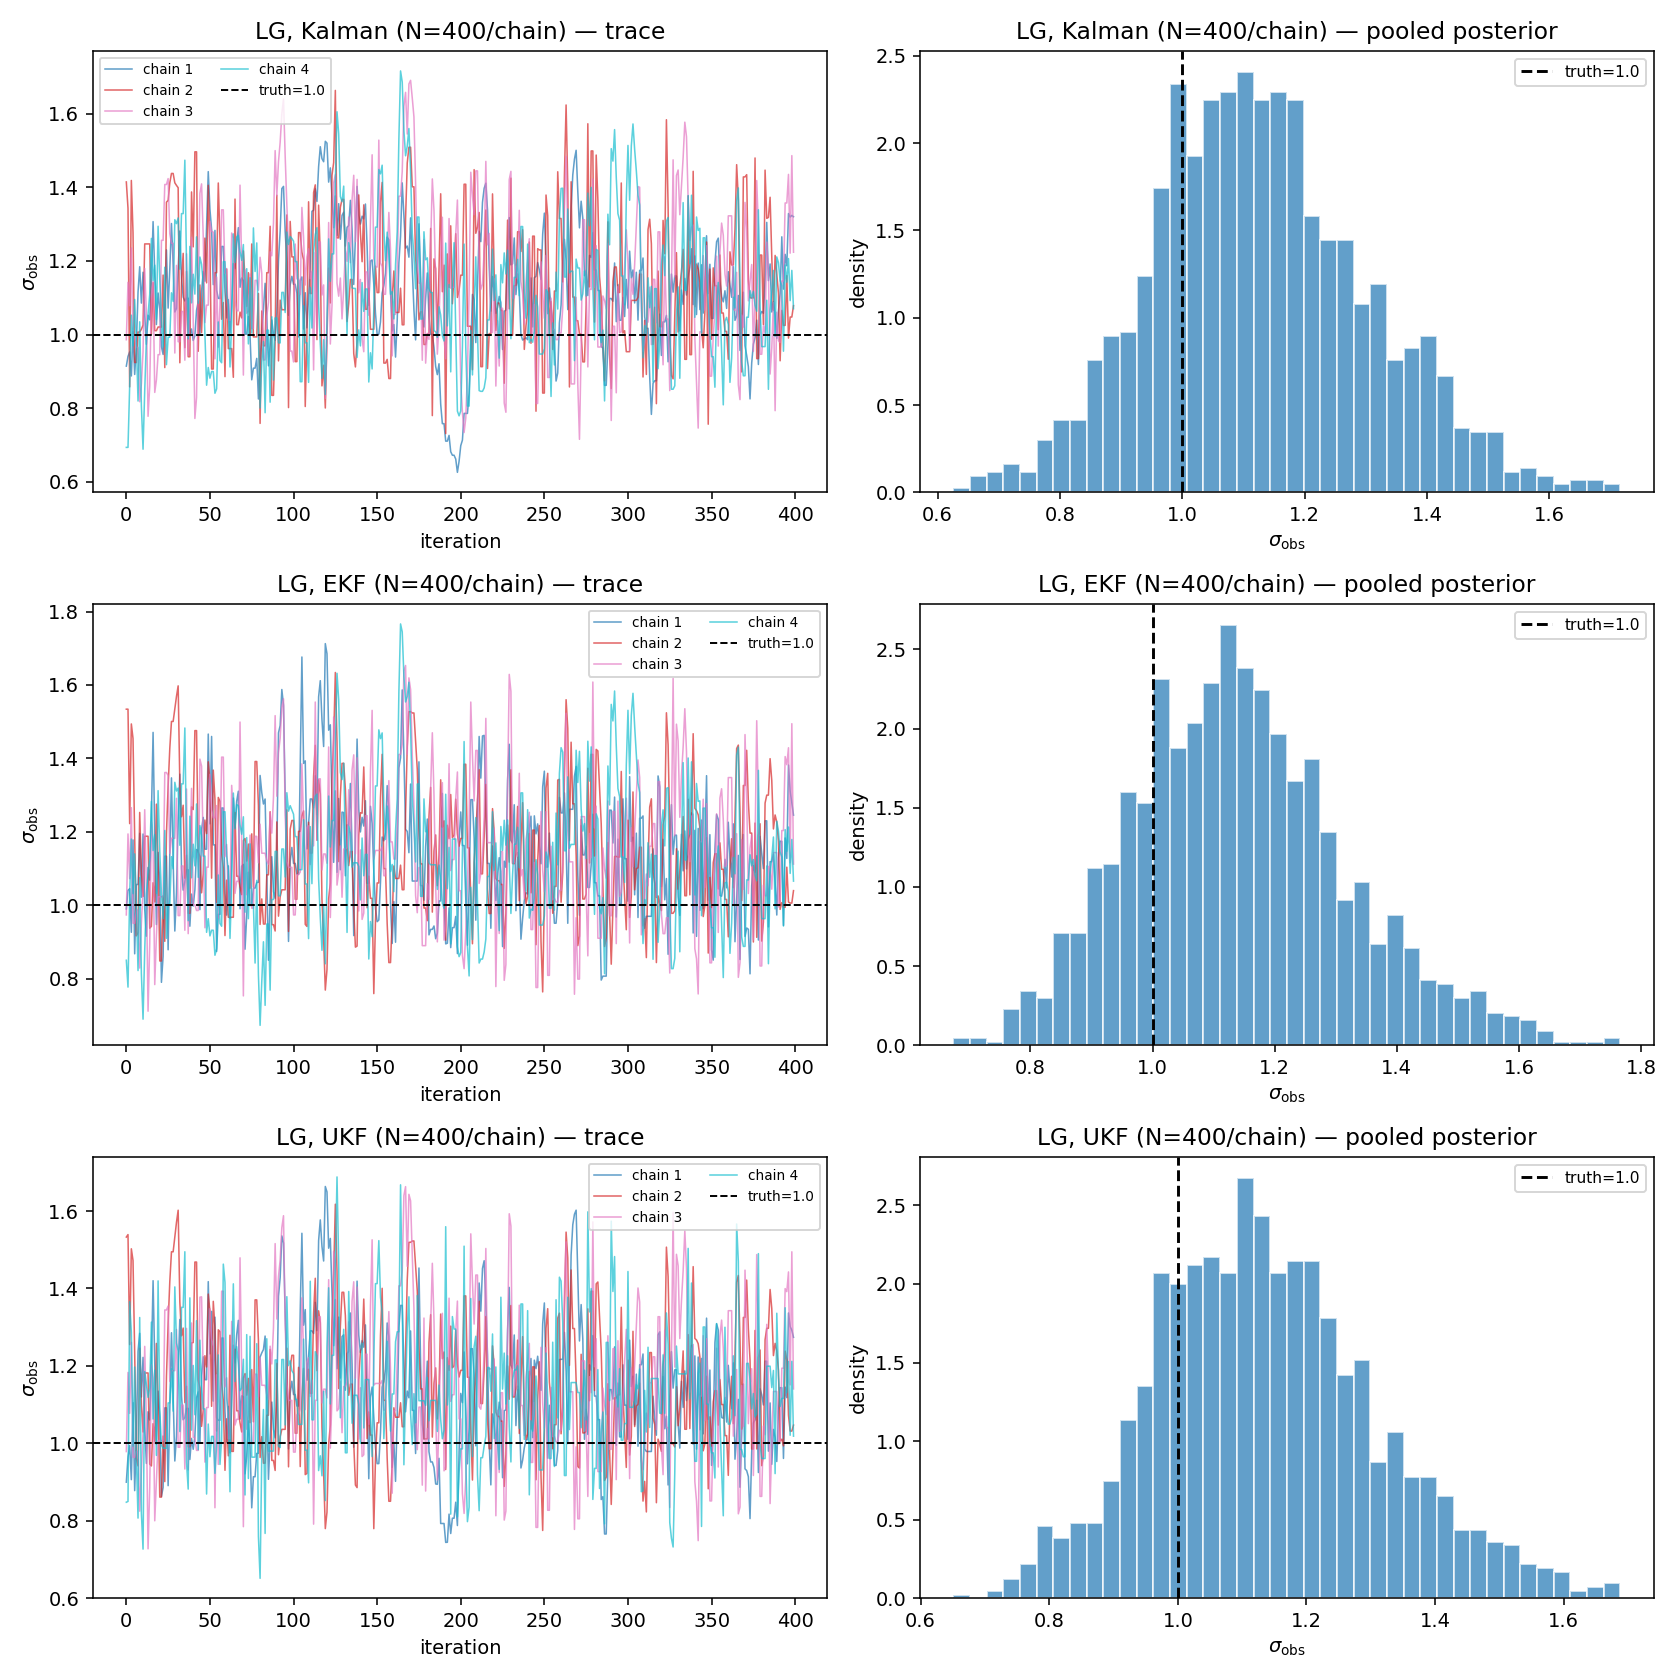
\includegraphics[height=0.62\textheight,keepaspectratio]{../report/figures/hmc_lg_kalman_family_4chain.png}
  \end{center}

  \medskip
  Posteriors from BPF$+$OT and LEDH$+$OT match the Kalman / EKF / UKF posteriors. $\hat R \le 1.01$, bulk + tail ESS $\ge 100$. The differentiable particle-filter pipeline reproduces the analytic answer on the model where the analytic answer exists.
\end{frame}

\begin{frame}{Benchmark step 4: HMC on SV1D}
  Stochastic volatility 1D, log-volatility latent $h_t$, observation $z_t = \exp(h_t/2)\, v_t$. No closed-form posterior. Recover $(\mu, \phi, \sigma_\eta)$ from $z_{1:T}$.

  \begin{center}
  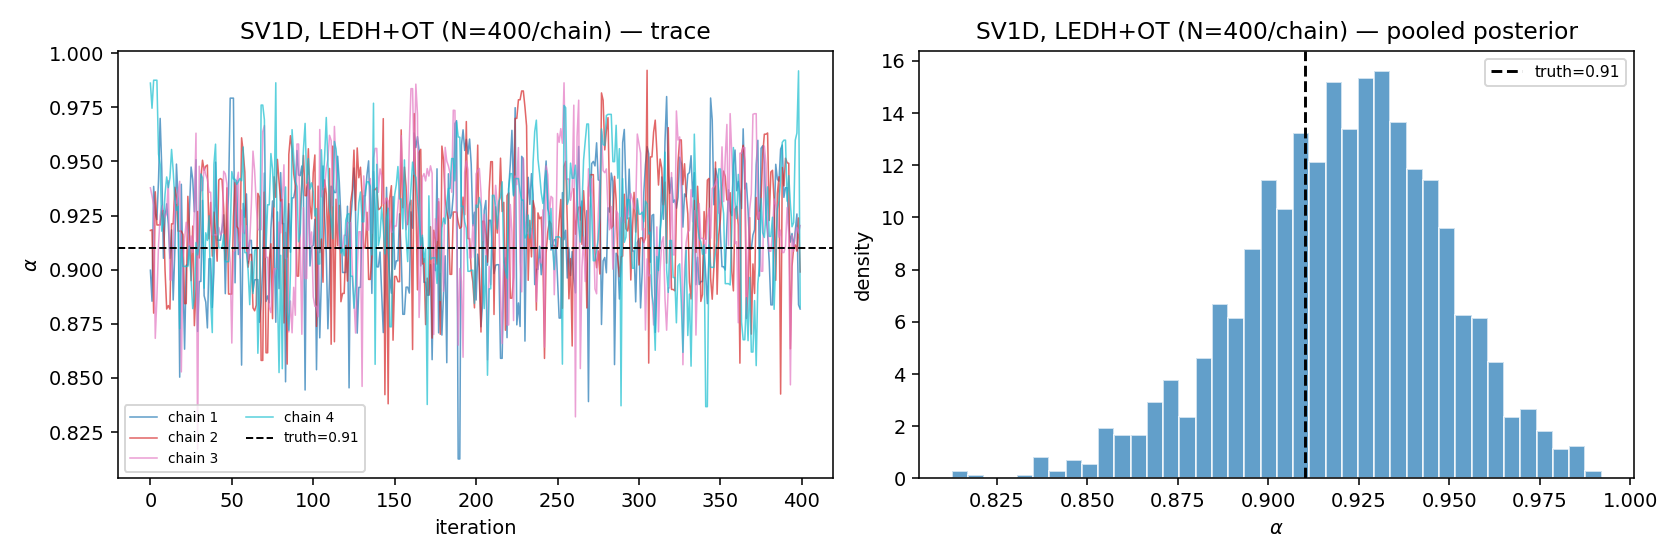
\includegraphics[width=0.78\linewidth]{../report/figures/hmc_sv1d_4chain_combined.png}
  \end{center}

  \medskip
  Four chains converge cleanly. Bulk + tail $\hat R \le 1.01$ across all three parameters. Posterior medians at the truth, contraction relative to prior visible.
\end{frame}

\begin{frame}{Profiling commitments}
  Before claiming any speedup:
  \begin{itemize}
    \item Profile a 10-leapfrog HMC window for LEDH$+$OT on the largest model in the benchmark set. Breakdown:
    \begin{enumerate}
      \item Flow accumulation $T \times n_\lambda \times N$
      \item Sinkhorn forward
      \item Implicit backward solve
      \item Parameter-Jacobian path
      \item Framework overhead
    \end{enumerate}
    \item Cross-check: 1D / 2D models are op-launch bound ($\sim 10\,\mu$s per op); only 5D$+$ shows true algorithmic scaling.
    \item Memory: confirm post-fix steady state. Earlier leak was 13--18 GB per call from particle initialisation inside the marginal-likelihood routine.
  \end{itemize}

  \medskip
  Measured XLA win: $\sim 1.3\times$ forward at $T{=}20$. \textbf{Do not promise more before measuring.}
\end{frame}

\begin{frame}{Identifiability when $z_t = A x_t + \dots$}
  \textbf{Scalar $a$:} clean. $a$ enters linearly in the mean, $\partial\!\log p/\partial a = (z_t - a x_t) x_t / R_t$. EKF / BPF / LEDH all work.

  \medskip
  \textbf{Matrix $A$ ($d \ge 2$):} $(A, x_t)$ identifiable only up to $(A Q^{-1}, Q x_t)$ for invertible $Q$. Fix by canonical form:
  \begin{itemize}
    \item Lower-triangular $A$ with positive diagonal --- easiest with a fill-scale-triL bijector.
    \item Stiefel manifold (orthonormal columns) --- needs manifold sampler.
    \item First entry of each column fixed to 1 --- factor-model loading normalisation.
  \end{itemize}

  \medskip
  Rank conditions: $\dim(y) > \dim(h)$ identifiable up to column rotation; $\dim(y) < \dim(h)$ leaves part of $h$ unobservable.
\end{frame}

\begin{frame}{Bonus: Hamiltonian Neural Networks}
  Idea (arxiv 2208.06120): train an HNN on $(\theta,\, \log p(y\given\theta),\, \nabla_\theta \log p)$ pairs from real HMC chains; use HNN-supplied $\nabla H$ in leapfrog instead of running the filter every step.

  \medskip
  \textbf{Why interesting.} Same amortisation argument as the OT operator, but at the \emph{posterior} level.

  \medskip
  \textbf{Why not now.}
  \begin{itemize}
    \item HNN needs accurate gradients --- noisy filter gradients in, garbage HNN out.
    \item Distributional shift: HNN generalises only inside training support; the posterior region is exactly what we don't know.
    \item Doesn't eliminate the filter --- still need MH correction with real $H$.
  \end{itemize}

  \medskip
  Future direction, not Phase-2.
\end{frame}

\begin{frame}[standout]
  Thank you
\end{frame}

\end{document}
